\documentclass[12pt]{article}
\usepackage{parskip}
\usepackage[nottoc]{tocbibind}
\usepackage{url}
\usepackage{float}

% center captions
\usepackage{caption}
\captionsetup{justification=centering}

% code
\usepackage{xcolor}
\usepackage{inconsolata}
\usepackage{xpatch}
\usepackage{realboxes}

\definecolor{numcolour}{HTML}{757575}
\definecolor{codegreen}{HTML}{428747}
\definecolor{backcolour}{HTML}{EDEDED}
\definecolor{codebrown}{HTML}{A34900}

\usepackage{listings}
\lstset{basicstyle=\ttfamily}

\lstdefinestyle{yaml}{
    numberstyle=\color{numcolour}\footnotesize\ttfamily,
    basicstyle=\color{black}\footnotesize\ttfamily,
    backgroundcolor=\color{backcolour},
    comment=[l]{\#},
    commentstyle=\bfseries\color{codegreen},
    string=[s]{"}{"},
    stringstyle=\color{codebrown},
    breaklines=true,
    numbers=left,
    showstringspaces=false,
    frame=single,
    captionpos=b
}

\lstdefinestyle{json}{
    numberstyle=\color{numcolour}\footnotesize\ttfamily,
    basicstyle=\color{codebrown}\footnotesize\ttfamily,
    backgroundcolor=\color{backcolour},
    string=[s]{"}{"},
    stringstyle=\color{codebrown},
    comment=[l]{:},
    commentstyle=\color{black},
    breaklines=true,
    showstringspaces=false,
    frame=lines,
    rulecolor=\color{black},
    numbers=left,
    captionpos=b
}



% highlighting
\usepackage{color}
\usepackage{soul}

% images
\usepackage{graphicx}
\graphicspath{ {./img/} }

\begin{document}

    \makeatletter
    \xpretocmd\lstinline{\Colorbox{backcolour}\bgroup\appto\lst@DeInit{\egroup}}{}{}
    \makeatother

    \begin{titlepage}
        \begin{center}
            \vspace{1cm}

            \LARGE
            Electronics and Computer Science\\
            Faculty of Physical Sciences and Engineering\\
            University of Southampton\\

            \Large
            \vspace{1.5cm}
            \textbf{Augustas Mirinas}\\
            \today

            \LARGE
            \vspace{1.5cm}
            \textbf{Trustless System for Personal Data Sharing}
            
            \vspace{1.5cm}
            \Large
            Project supervisor: Dr George Konstantinidis\\
            g.konstantinidis@soton.ac.uk
            
            \Large
            Second examiner: Dr Mark Vousden\\
            m.vousden@soton.ac.uk
            
            \vfill
            A project report submitted for the award of\\
            BSc Computer Science
            
        \end{center}
    \end{titlepage}

    \section*{Abstract}
    

    \newpage
    \tableofcontents


    \newpage
    \section{Design}

    \subsection{Data privacy}
    \label{subsec:privacy}

    % data publishing
    In this project, data privacy is achieved using an algorithm to compute "consent-abiding query answers" from the publication of the supervisor of this project \cite{konstantinidis}. In this publication, to ensure that parts of private data, not consented to share, will stay private, data queries are rewritten in compliance with data subject constraints. These constraints consist of rules specifying combinations of data fields that are prohibited from sharing. Each data subject has their own set of constraints, which is used as neccessary when rewriting data queries. After rewriting, resulting queries would only return data that is consented for sharing. To adapt this method for a trustless system - in which all network participants are able to reach an agreement about the past and current state of shared private information - constraints are used to filter shared data instead of rewriting data queries, as done in \cite{konstantinidis}. This makes the logic of consent-abiding data sharing independent from any private information publisher, as the data during publishing is filtered by the system, not by the publisher.

    % filtering and constraints
    In order to publish private information, it has to be linked to existing user (data subject) constraints, which are identified by a unique username. If a user of the information being published does not exist, the information will not be saved to the system. To create a user identity, data subject must come up with a username that does not exist in the system yet and submit it through an independent party. \hl{This independent party could be a government body or other data protection authorities, but it is not in the scope of this project.} At the same time user identity is created, user consent constraints are defined using an index of the information as a reference, as the data is published in the form of a table.

    % index and table format
    Both constraints and the index of data conforms to the table format. A single constraint is expressed as a combination of columns from the index - an example can be seen in Figure \ref{fig:constraints}, which is taken from \cite{konstantinidis}. The data being published contains records, or rows, with a username column to specify which user this record belongs to. \hl{The index, listing all possible columns of the record, is also uploaded by the user at the time of creating a constraint.} Only then can the data about this user, collected by some organization, be published to the system allowing authorised members of the network to access it, without compromising data subject's consent.

    \begin{figure}[H]
        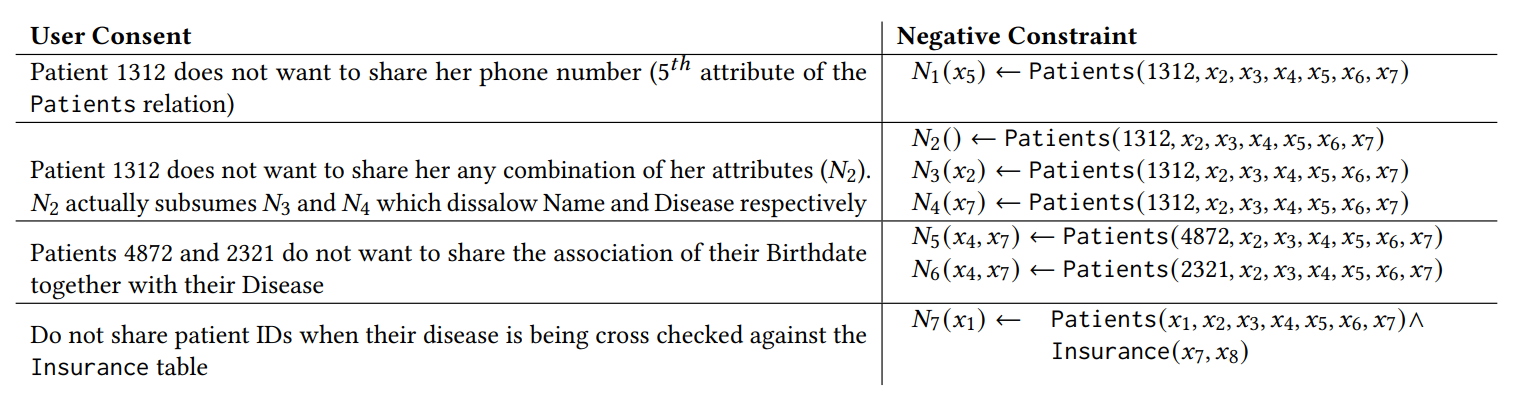
\includegraphics[width=\textwidth]{constraints.png}
        \caption{A capture of the table showing some examples of user constraint semantics}
        \label{fig:constraints}
    \end{figure}

    
    % https://www.youtube.com/watch?v=Dki-WetBmAY&ab_channel=DraeganNetwork

    \subsection{Blockchain}
    \subsubsection{Motivation}
    The design chosen for this project relies on blockchain technology - utilising decentralisation and immutability to create a system, where shared information cannot be manipulated and is maintained by every permissioned member of the network. Traditionally, sensitive user information for sharing is pooled into a single place, then accessed by different parties as needed. \hl{Add a reference to a centralised HIE implementation.} This presents a challenge to match different pieces of data from different sources to form correct user profiles. User identification, data formats and privacy concerns are considered when applying advanced algorithms to solve this problem. A decentralised blockchain network addresses these problems more efficiently and with better reliability - network members have access and can participate only when they are following policies set and agreed by the rest of the network.

    % blockchain ledger
    To enforce the network policies on the participants, the system produces a record of every network member interaction. These records, containing information about the interaction and ordered based on the interaction timestamp, form a public ledger. Member interactions with the system are also called transactions. Only transactions, approved by required members are valid and recorded into a ledger. The ledger is replicated across multiple network members to prevent any unauthorised changes to the ledger - if a malicious member would attempt to change the record of system transactions, other network members would still be able to agree on the correct ledger version and deny the unauthorised change, based on their ledger replicas. This results in a system that consists of multiple independent members following the same rules and policies. This feature of the blockchain network is used for implementation of the data privacy algorithm presented in subsection \ref{subsec:privacy}.

    % decentralised data storage
    One major advantage of a blockchain network over a traditional centralised information exchange approach is data storage. The proposed blockchain network does not store data on the ledger, nor does it communicate private information through transactions - meaning actual data intended for sharing is never recorded on the public ledger. Instead, when publishing new data to the system only the hash of data is made public. Actual private data is stored only by the data publisher and any members that have access to it. This model records evidence of published data and makes it public to everyone without revealing the contents of published data. By inspecting hashes of data in the ledger, it is possible to confirm private data was not tampered with after publishing. This and more scenarios will be analysed in section \ref{sec:scenarios}. Another benefit of fragmented data storage is damage mitigation in case of a data breach or a malicious access. A member of the network will only store information that is either used or published by themselves - in most cases this will be a small subset of overall private data published to the system, which means a single instance of a data breach would compromise less private information than in the traditional centralised data exchange, where all private information is pooled to a single place.

    % consensus mechanism
    \subsubsection{Network design}
    The blockchain network implementing this design is permissioned, meaning every member of the network is known and has defined access to resources and permissions to commit certain transactions. This is different from public blockchain systems, such as Bitcoin\cite{bitcoin} or Ethereum\cite{ethereum}, where unknown members can be part of the network and their transactions are validated via "proof of stake" or other consensus mechanisms. The task of transaction validation of a permissioned blockchain network is designated to a trusted provider of this service - a member of the network with the role of deciding which transactions are valid and should be recorded into the ledger. The same network node is also responsible for issuing and identifying members of the system. \hl{This method of transaction validation and member identification is more scalable and provides additional features to the network, compared with "proof of stake" and similar mechanisms (provide reference for this statement?)}

    
    % network components
    The second component to be implemented after the network validator is a channel. This network component defines which network members are able to participate in the channel, how transactions of the channel should be approved and who can make and approve changes to the channel configurations. These configurations may vary depending on the use case of this system - some examples will be given in section \ref{sec:scenarios}. For each channel, a set of functions are defined in smart contracts of the blockchain network. These functions implement private data filtering using user constraints and enable data publishing, reading and constraint registering. Furthermore, smart contracts define collections of data and which members can read or write to those collections. These network components allow highly customizable segmentation of information access. Different areas of information could be separated into channels - each one would have an individual ledger for better scalability and collections would be used to control access for different members of the network.


    \section{Implementation}

    To implement this blockchain system for secure and consent-abiding private data sharing Hyperledger Fabric will be used - an "open source enterprise-grade permissioned distributed ledger technology platform"\cite{fabric}. This technology was established under the Linux Foundation, which has a reputable history of open source projects. Hyperledger Fabric is a permissioned blockchain system, meaning every member of the network knows each other. This is well suited for a proposed design, as all members - either data subjects, data publishers or data users - should be approved anyway. Every member of the system has the same goal - provide useful information or use it for a good cause. Any action is recorded on a ledger, deterring any malicious members to take action and face consequences.

    \subsection{Environment and tools}
    \label{subsec:environment}
    The deployment of this implementation is not production grade - to ease development process, explanation of the system and to allow easy replication for anyone interested, all network components are deployed on a single machine. Docker Compose is used for this purpose - by defining a \lstinline{docker-compose.yaml} file, multiple containers are brought up using officialy supported Hyperledger Fabric commands. These commands use environment variables and generated network certification files to correctly set up nodes of the network. In production environment, these files and variables should be carefully considered for each component of the network, but in this project the Docker Compose configuration and other required files are going to be generated by Fablo - "a simple tool to generate the Hyperledger Fabric blockchain network"\cite{fablo}. Fablo takes one configuration file as an input and generates the network with specified organizations and other neccessary components. Then \lstinline{fablo} commands can be used to manage the generated network. This tool is part of Hyperledger Labs - a space to start and contribute to projects related to Hyperledger Fabric. Another tool from the same origin is Blockchain Explorer\cite{explorer}, useful for observing transactions made on the network using graphical user interface. Java with Maven is used for developing smart contracts and Git for version control.

    \subsection{Network configuration}
    In Hyperledger Fabric, the node validating blockchain network transactions is called an orderer. Here, orderer is hosted by a regulating authority - a trusted third party. Other network components are 3 organizations - separate business entities, publishing and/or using private data collected from users (data subjects). Fourth organization is responsible for consensus of data subjects. Through this organization, users can submit their consent constraints, which will be used to only publish information consented for sharing. Each organization is only a logical unit; to interact with the network, each organization will have one physical network node, called peer in Hyperledger Fabric. As stated in subsection \ref{subsec:environment}, network configuration files and required environment variables will be generated with the help of Fablo, therefore in this section Fablo configuration file will be demonstrated, which is more concise and easier to explain compared to many files, required for the Fabric network. Here, only a part of the configuration file will be shown with comments to explain each setting.

    \newpage
    \begin{lstlisting}[style=yaml,
        caption={fablo.yaml - configuration file generating the network}, label={lst:network}]
---
# global network settings
global:
    fabricVersion: "2.5.0"
    # enable TLS for secure communication between network nodes
    tls: "true"
    tools:
        # start a Node.js server hosting Blockchain Explorer
        explorer: "true"
orgs:
    # orderer organization, hosting a node which validates transactions
    - organization:
        name: "Orderer"
        domain: "orderer.org"
        orderers:
          - prefix: "orderer"
            type: "raft"
            # can be more than one orderer node for redundancy
            instances: 1
    # data publisher, user or consenter organization
    - organization:
        name: "Org1"
        mspName: "Org1MSP"
        domain: "org1.co"
        ca:
            prefix: "ca"
        peer:
            prefix: "peer"
            # multiple nodes could be used to have multiple data points in the organization
            instances: 1
            db: "LevelDb"

    # ...
    # three more organizations are defined but omitted with identical settings
    # org2.ac - publisher/user
    # org3.gov - publisher/user
    # owners.org - data subjects (consenters)
    # ...
    
channels:
    # one channel consisting of all organizations defined
    - name: "ch1"
        orgs:
          - name: "Org1"
            peers:
              - "peer0"
          - name: "Org2"
            peers:
              - "peer0"
          - name: "Org3"
            peers:
              - "peer0"
          - name: "Owners"
            peers:
              - "peer0"
    \end{lstlisting}

    After generating the network using given configuration in listing \ref{lst:network}, all nodes are created and started. As mentioned, each organization has its own peer, which can interact with the network. Organization \lstinline{mspName} can be used to control resource access in smart contracts - this is used when granting access to create consent constraints for \lstinline{owners.org} organization. Another option for organization is database implementation. Every node has an instance of database, where network data, such as consent constraints or published user information, is stored and queried from. Any changes in network data is propagated in databases of each node. Option \lstinline{db} specifies whether to use LevelDb or CouchDb for peer database implementation. LevelDb is used for this project, utilising its flexibility and speed. Data is stored as ordered key-value pairs, and maps string keys to byte array values, meaning any information can be stored, as long as it can be deterministically serialized into bytes. CouchDb is a NoSQL database storing data as JSON objects, which runs as a separate database process and enables rich queries, however it is left for future considerations. Lastly, a single channel is defined consisting of peers of every organization defined. In figure \ref{fig:network}, all spawned Docker containers and Hyperledger Fabric commands used to start them are shown.
    
    \begin{figure}[H]
        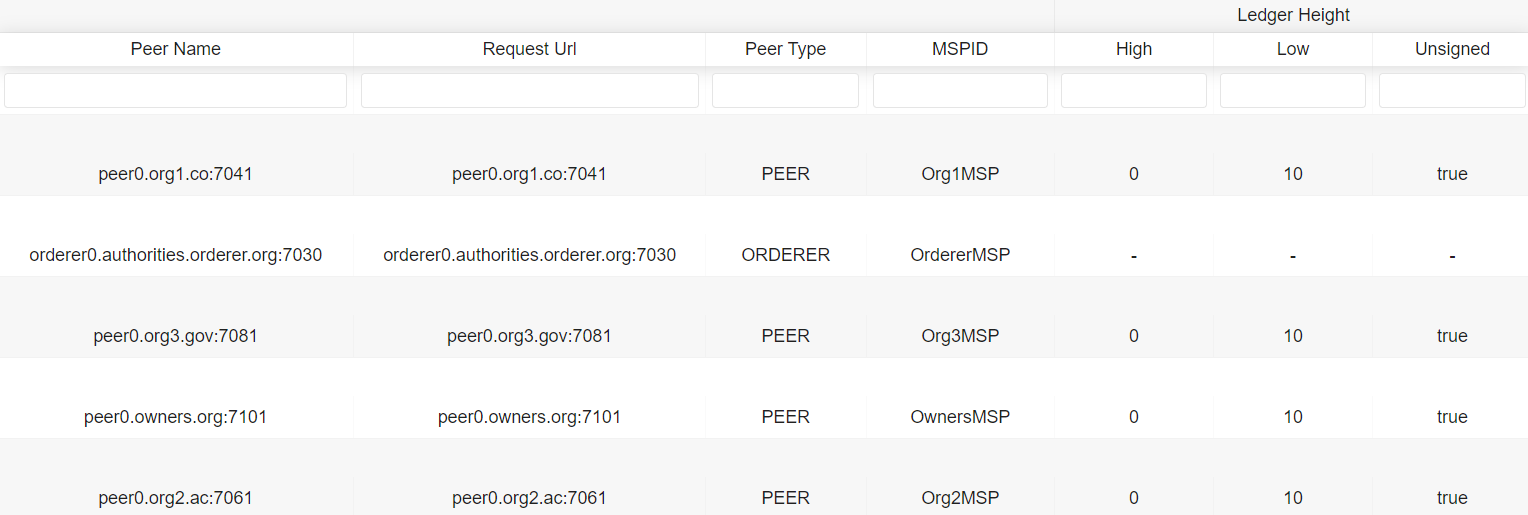
\includegraphics[width=\textwidth]{network.png}
        \caption{A Blockchain Explorer table listing all network components}
        \label{fig:network}
    \end{figure}


    \subsection{Chaincode}
    In figure \ref{fig:network}, ledger height can also be seen. Height of 10 means 10 blocks have been appended to the ledger. Some appended blocks contain a channel configuration transaction. Fabric commands, such as \lstinline{configtxgen}, \lstinline{peer channel create} and \lstinline{peer channel join} are used by Fablo to produce these transactions, creating a channel and joining all peers in result. Other blocks contain endorsement transactions, which are produced with \lstinline{peer lifecycle chaincode} commands. These commands install chaincode to the Fabric network. Chaincode defines smart contracts, which have a set of functions, that describe what actions can be executed in the network. Every chaincode also has an endorsement policy, indicating which organizations have to endorse a smart contract invoke (a transaction) for that transaction to be valid and for the smart contract function to change the state of the public ledger. Endorsement policies are agreed at the time of chaincode instalation and they are applied for every chaincode invoke. Chaincode with endorsement policies is defined in \lstinline{fablo.yaml} - the configuration file from listing \ref{lst:network}. In listing \ref{lst:chaincode}, a continuation of the file is shown.

    \newpage
    \begin{lstlisting}[style=yaml,
        caption={fablo.yaml - configuration file defining network chaincode}, label={lst:chaincode}]
---
global:
    # ...
orgs:
    # ...
channels:
    # ...
chaincodes:
  - name: "private-data"
    version: "1.0"
    # language that the chaincode is written in
    lang: "java"
    # channel that will get this chaincode installed
    channel: "ch1"
    # physical files of the chaincode
    directory: "private-data-chaincode"
    # endorsement policy - all organizations are required to endorse this chaincode and its invokations
    endorsement: "OR('Org1MSP.member', 'Org2MSP.member', 'Org3MSP.member')"
    # private data collections shared with different organizations to controll private information access
    privateData:
      - name: "CollectionA"
        orgNames:
            - "Org1"
            - "Org3"
      - name: "CollectionB"
        orgNames:
            - "Org1"
            - "Org2"
            - "Org3"
      - name: "CollectionC"
        orgNames:
            - "Org2"
            - "Org3"
    \end{lstlisting}


    % all orgs endorse - cc install, cc change
    % cc works only on one channel - other channel ccs can have different endorsement
    % private data collections - what can be stored in a collection, how are they separated
    % private data collections have overrulling endorsement policy
    In this implementation, one smart contract is endorsed by all organizations in the network




    \section{Example scenarios}
    \label{sec:scenarios}

    % malicious publisher
    % malicious reader
    % no 3rd org

    \subsection{Private data tampering}




    
    
    \newpage
    \bibliographystyle{ieeetr}
    \bibliography{refs}

\end{document}
